
\documentclass[11pt, spanish]{report}
\usepackage[spanish]{babel}
\usepackage[utf8]{inputenc}
\usepackage{geometry}
 \geometry{
 a4paper,
 total={170mm,257mm},
 left=20mm,
 top=20mm,
 }
\usepackage{graphicx}
\graphicspath{ {images/} }
% Aquí comienza el contenido


\title{Información climática}
\author{César Andrés Pérez Robinson }
\date{February 2019}

\begin{document}

\maketitle

\section{Introducción}
A continuación se presenta una serie de actividades realizadas para aprender a utilizar "jupyter notebook", las actividades estuvieron relacionadas a la creación de tablas y gráficas estadísticas sobre datos climáticos de una ciudad de la República. En el caso particular del presente trabajo, se presentan los datos obtenidos por la página http://smn1.conagua.gob.mx/emas/ de la ciudad de Cancún desde Enero 23 a Enero 29 del 2019. 
\section{Procedimiento}
A continuación se presentan los pasos que se utilizaron en "jupyter notebook" para concluir la actividad. \\
\emph{Entrada} [1]; Se descarga Pandas, para el manejo de datos y se le asigna las letras \emph{pd} de manera que al usarse solo basta con utilizar \emph{pd}. Mismo procedimiento con numpy y matplolib.
\begin{verbatim}
    # Cargar a la memoria de trabajo las bibliotecas: Pandas (manejo de datos, 
    # Numpy (numerical python) y la biblioteca de gráficas Matplotlib
    # Se asignan nombres cortos.
    import pandas as pd
    import numpy as np
    import matplotlib.pyplot as plt
    #
    # Usar "Shift+Enter" para procesar la información de la celda
\end{verbatim}

\emph{Entrada} [2]; Se descargaron los datos de la estación del Servicio Meteorológico Nacional en \\ http://smn1.conagua.gob.mx/emas/ de Cancún.
\begin{verbatim}
    df0 = pd.read_csv('cancun.txt', skiprows=4, sep='\s+')
\end{verbatim}

\emph{Entrada} [3]; Se piden los primeros cinco renglones del texto y se obtiene la Figura 1.  
\begin{verbatim}
    df0.head()
\end{verbatim}
\begin{figure}[h]
\caption{Primeros cinco renglones de texto}
\centering
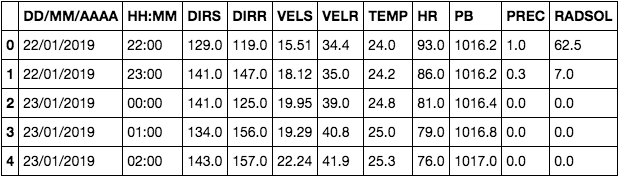
\includegraphics[width=\textwidth]{primeros5.png}
\end{figure}

\emph{Entrada} [4]; Se le da una estructura de datos.  
\begin{verbatim}
    df = pd.DataFrame(df0)
\end{verbatim}
\emph{Entrada} [5]; Se ven los tipos de datos que Pandas ha reconocido al leer.  
\begin{verbatim}
    df.dtypes

    Out[5]
      DD/MM/AAAA     object
      HH:MM          object
      DIRS          float64
      DIRR          float64
      VELS          float64
      VELR          float64
      TEMP          float64
      HR            float64
      PB            float64
      PREC          float64
      RADSOL        float64
      dtype: object
\end{verbatim}
\emph{Entrada} [6]; A continuación convierte una variable de tiempo, combinando las columnas \\ DD/MM/AAAA con HH:MM para crear la nueva columna FECHA, la cual se presenta en un formato de tiempo. Adicionalmente, se eliminan las dos columnas anteriores.
\begin{verbatim}
    df['FECHA'] = pd.to_datetime(df.apply(lambda x: x['DD/MM/AAAA'] + ' ' + 
    x['HH:MM'], 1), dayfirst=True)
    df = df.drop(['DD/MM/AAAA', 'HH:MM'], 1)
\end{verbatim}

\emph{Entrada}[7]; Utilizando el comando anterior para obtener los primeros cinco reglones del texto, observamos en la Figura 2 que las variables de DD/MM/AAAA y HH:MM se han eliminado y se ha creado la variable FECHA.
\begin{verbatim}
    df.head()
\end{verbatim}
\begin{figure}[h]
\caption{Primeros cinco renglones de texto, con variable FECHA}
\centering
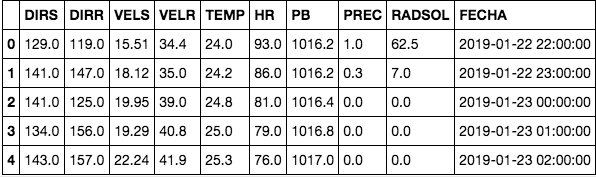
\includegraphics[width=\textwidth]{primero5x.png}
\end{figure}

\emph{Entrada}[8]; Realizando un análisis exploratorio de datos obtenemos la Figura 3.
\begin{verbatim}
    df.describe()
\end{verbatim}
\begin{figure}[h]
\caption{Análisis exploratorio de datos}
\centering
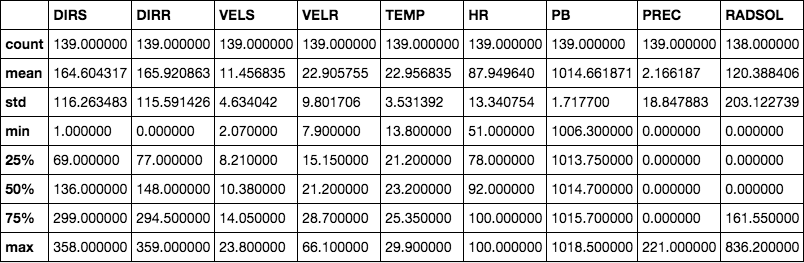
\includegraphics[width=\textwidth]{datos.png}
\end{figure}

\emph{Entrada}[8]; Podemos seleccionar un apartado específico de datos, por ejemplo, aquellos datos en los cuales la Temperatura era mayor a $24^\circ C$ y menor a $25^\circ C$, lo que se muestra en la Figura 4.
\begin{verbatim}
   # Selecciona los renglones con Temperatura > 24ºC y < 25ºC
    df_tmp = df[df.TEMP > 24] 
    df_select = df_tmp[df_tmp.TEMP < 25]
    df_select 
\end{verbatim}
\begin{figure}[h]
\caption{Temperatura $>\ 24^\circ C \ y \ < \ 25^\circ C$}
\centering
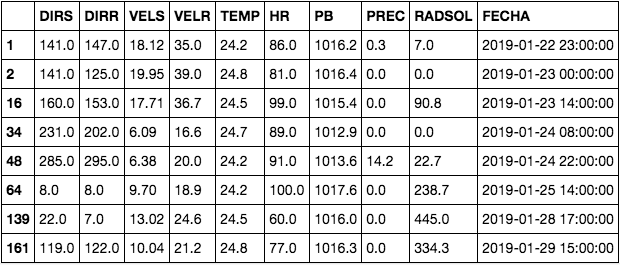
\includegraphics[width=\textwidth]{temp24-25.png}
\end{figure}

\emph{Entrada}[9]; Podemos calcular el promedio de todas las columnas utilizando:
\begin{verbatim}
    df.mean()
Out[9]
    DIRS       164.604317
    DIRR       165.920863
    VELS        11.456835
    VELR        22.905755
    TEMP        22.956835
    HR          87.949640
    PB        1014.661871
    PREC         2.166187
    RADSOL     120.388406
    dtype: float64
\end{verbatim}

\emph{Entrada}[10]; O calculando específicamente una de las columnas, como Temperatura.
\begin{verbatim}
    df.TEMP.mean()
Out[13]:
    22.9568345323741
\end{verbatim}

\emph{Entrada}[10]; Graficando la rapidez de los vientos en $\frac{m}{s}$, obtenemos la Figura 5.
\begin{verbatim}
    plt.figure(); df.VELS.plot(); plt.legend(loc='best')
    plt.title("Variación de la Rapidez de los Vientos")
    plt.ylabel("Rapidez (m/s)")
    plt.grid(True)
    plt.show()
\end{verbatim}
\begin{figure}[h]
\caption{Variación de la rapidez de los vientos}
\centering
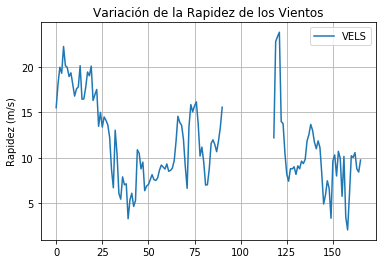
\includegraphics[width=0.65\textwidth]{rapidez.png}
\end{figure}

\emph{Entrada}[11]; Graficando la Temperatura y la Humedad Relativa se obtiene la Figura 6.
\begin{verbatim}
    df1 = df[['TEMP','HR']]
    plt.figure(); df1.plot(); plt.legend(loc='best')
    plt.title("Variación de la Temperatura y la Humedad Relativa")
    plt.ylabel("Temp ºC /(%) HR")
    plt.grid(True)
    plt.show()
\end{verbatim}
\begin{figure}[h]
\caption{Temperatura y Humedad Relativa}
\centering
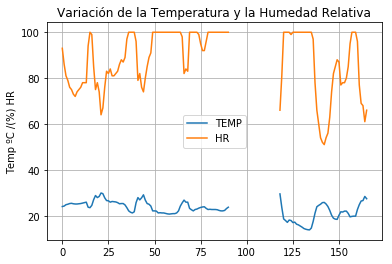
\includegraphics[width=0.65\textwidth]{Temphum.png}
\end{figure}

\emph{Entrada}[12]; Graficando la variación de Temperatura en función del tiempo en la Figura 7.
\begin{verbatim}
    plt.plot_date(x=df.FECHA, y=df.TEMP, fmt="b-")
    plt.title("Variación de la Temperatura")
    plt.ylabel("Temp ºC")
    plt.grid(True)
    plt.show()
\end{verbatim}
\begin{figure}[h]
\caption{Temperatura y Humedad Relativa}
\centering
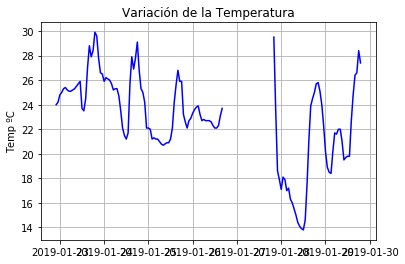
\includegraphics[width=0.65\textwidth]{temptiem.png}
\end{figure}

\emph{Entrada}[13]; Creando una gráfica que nos muestra la rapidez de los vientos y de las ráfagas en función del tiempo en la Figura 8. La hora donde se presentó la mayor velocidad del viento fue a las 11:00 PM del dia 27, sin embargo la mayor rapidez de las ráfagas fue obtenida a las 9:00 del mismo día.
\begin{verbatim}
    trace1 = go.Scatter(
        x=df.FECHA,
        y=df.VELS,
    name='Rapidez de los vientos',
   
    )
    trace2 = go.Scatter(
        x=df.FECHA,
        y=df.VELR,
    name = 'Rapidez de las ráfagas ',
    )

    data = [trace1, trace2]

    fig = dict(data=data)
    py.iplot(fig, filename='simple-connectgaps')
\end{verbatim}
\begin{figure}[h]
\caption{Rapidez de Vientos y Ráfagas}
\centering
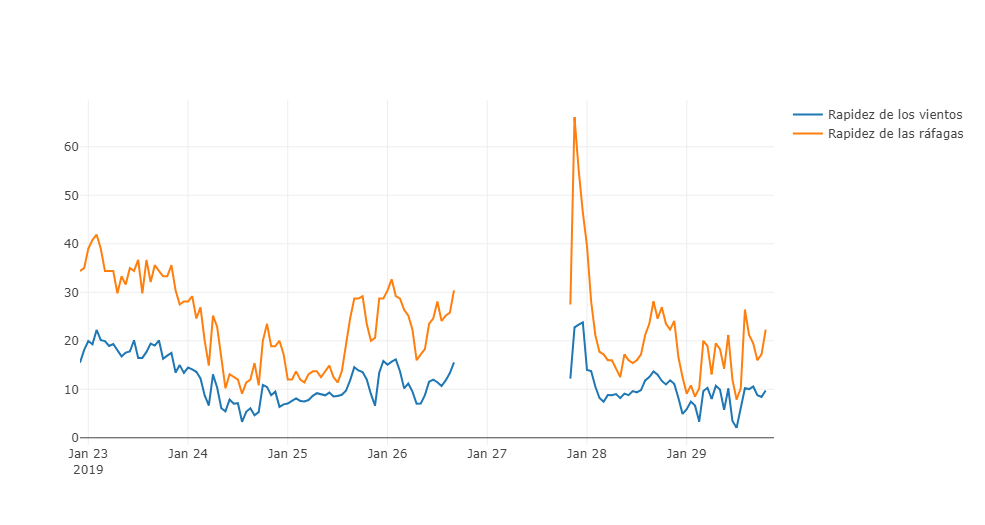
\includegraphics[width=\textwidth]{vientosrafagas.png}
\end{figure}

\emph{Entrada}[14]; Para graficar la dirección de los vientos junto con la velocidad de los mismos en función a la fecha en la Figura 9, primero se creó una nueva variable VELS2, la cual representa la velocidad de los vientos multiplicada por 10, con la finalidad de que ambos trazos se ubicaran dentro de los mismos rangos numéricos. 
\\
La velocidad de los vientos más alta fue la registrada a las 11:00 el 27 de Enero, cuya dirección se orientaba a $13^\circ$ del Norte
\begin{verbatim}
    df['VELS2']=10*(df.VELS)
    
    trace1 = go.Scatter(
        x=df.FECHA,
        y=df.DIRS,
        name='Dirección',
    )
    trace2 = go.Scatter(
        x=df.FECHA,
        y=df.VELS2,
        name = 'Intensidad ',
    )
    data = [trace1, trace2]
    fig = dict(data=data)
    py.iplot(fig, filename='simple-connectgaps')
\end{verbatim}
\begin{figure}[h]
\caption{Dirección de los vientos}
\centering
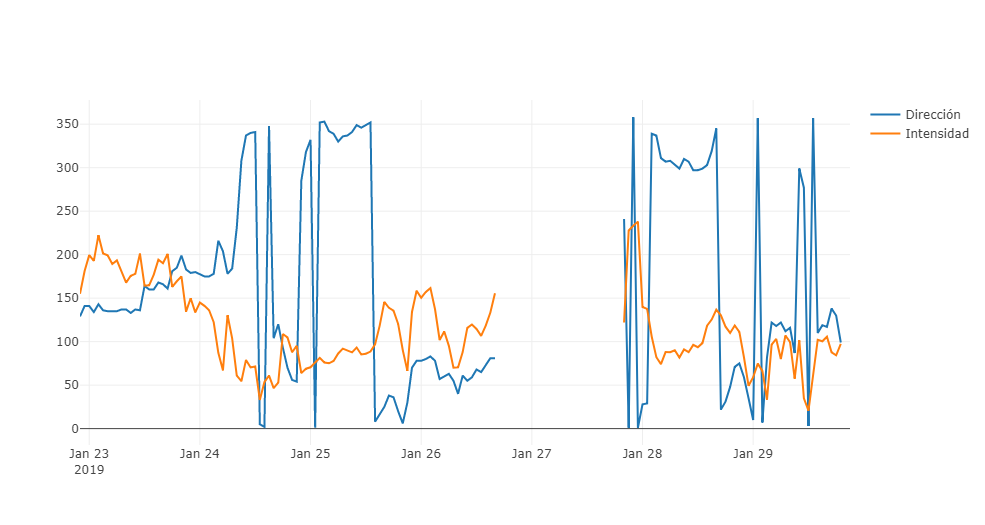
\includegraphics[width=0.80\textwidth]{direccion.png}
\end{figure}


\emph{Entrada}[15]; Se analiza la radiación solar registrada en la Figura 10. Obviamente la radiación solar es nula en los horarios de la noche, por lo que la gráfica muestra momentos donde la radiación solar es igual a 0.
\begin{verbatim}
    trace = go.Scatter(
    x=df.FECHA,
    y=df.RADSOL,
    name='Radiación Solar',
    )
    data = [trace]
    fig = dict(data=data)
    py.iplot(fig, filename='simple-connectgaps')
\end{verbatim}
\begin{figure}[h]
\caption{Radiación Solar}
\centering
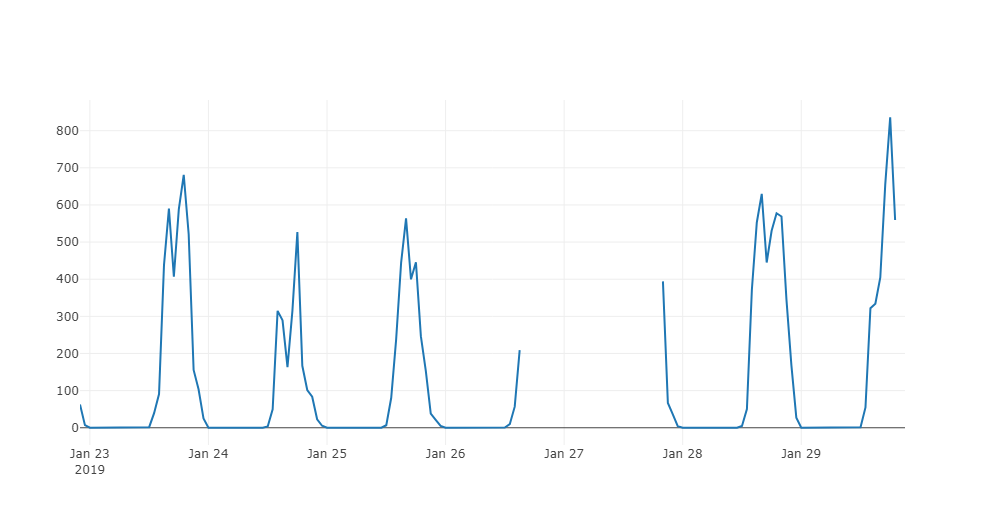
\includegraphics[width=0.80\textwidth]{radsol.png}
\end{figure}

\emph{Entrada}[16]; El lapso presentado en los datos obtenidos es de $16.09^\circ$C, lo cual fue obtenido a partir de restar la temperatura mínima a la temperatura máxima con la entrada:
\begin{verbatim}
    df.TEMP.max()-df.TEMP.min()
\end{verbatim}

\section{Comentarios}
Las impresiones al utilizar jupyter notebook son positivas, como lo es en la mayoría de las cosas, al inicio se debe de ajustarse a la sintaxis y a las restricciones que presenta, sin embargo, una vez entendiendo el procedimiento y sabiendo donde buscar información, es fácil de usar, la creación de gráficas interactivas es muy eficiente y sin duda utilizaré el programa de nuevo para la realización de distintos trabajos.
\\
Me pareció similar a Fortran, al declarar y llamar una variable, el hecho de que en Phyton se tiene que importar el programa que deseas utilizar y asignar una manera de cómo será llamado y utilizado en el futuro.
\\
No me pareció que la actividad fuera difícil, es normal en cualquier situación el tener una curva de aprendizaje y sentir que no se está avanzando en nada, pero el saber donde y como buscar información en internet para poder completar la actividad es la manera en que se logra el objetivo.



\end{document}